\documentclass[a4paper,1pt]{report}
\usepackage[utf8]{inputenc}
\usepackage[spanish]{babel}
\usepackage{amsfonts}
\usepackage{amsthm}
\usepackage{amssymb}
\usepackage{amsmath}
\usepackage{graphicx}
\usepackage{subcaption}
\usepackage{float}
\usepackage[rightcaption]{sidecap}

\newtheorem*{pbo}{Principio del Buen Ordenamiento}

\newtheorem*{pim}{Principio de Inducción Matemática}

\newtheorem*{teo}{Teorema}

\newtheorem*{cor}{Corolario}

\newtheorem*{dem}{Demostración}

\newtheorem*{dfn}{Definición}

\newtheorem*{lem}{Lema}

\newtheorem*{prp}{Propiedades}


% Title Page
\title{Conferencia 8 - Grafos Dirigidos}
\author{}

\begin{document}
\maketitle

\begin{dfn}
 Un \textbf{grafo dirigido}~(digrafo) consiste en dos conjuntos $V$, el conjunto de los nodos, y $E$, el conjunto de los arcos, formado ahora por pares ordenados del conjunto $V$.
\end{dfn}

\begin{figure}[H]
    \centering
    \begin{subfigure}[b]{0.80\textwidth}
        \centering
        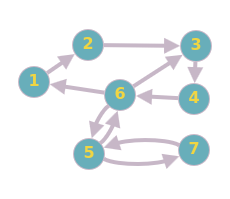
\includegraphics[width=0.4\textwidth]{figures8/digrafo.png}
    \end{subfigure} 
    \caption{Ejemplo de Digrafo}
\end{figure} 

\begin{dfn}
 Sean $v,w\in V(G)$ donde $G$ es un digrafo, $v,w$ son adyacentes si el arco $<v,w>\in E(G)$ o si el arco $<w,v> \in E(G)$. Si $<v,w> \in E(G)$ se dice que el arco $<v,w>$ es incidente desde $v$ y que es incidente a $w$.
\end{dfn}

\begin{dfn}
 Sea $G$ un digrafo y $v\in V(G)$:
 \begin{itemize}
  \item El grado exterior de $v$ es el número de arcos incidentes desde $v$~(exdeg(v) o outdeg(x)).
  \item El grado interior de $v$ es el número de arcos incidentes sobre $v$~(indeg(v)).
 \end{itemize}
\end{dfn}

\begin{figure}[H]
    \centering
    \begin{subfigure}[b]{0.45\textwidth}
        \centering
        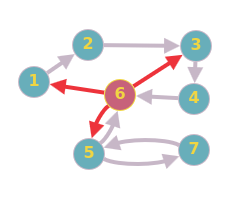
\includegraphics[width=0.7\textwidth]{figures8/outdeg.png}
        \caption{$outdeg(6) = 3$}
    \end{subfigure} 
        \begin{subfigure}[b]{0.45\textwidth}
        \centering
        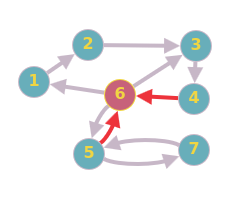
\includegraphics[width=0.7\textwidth]{figures8/indeg.png}
        \caption{$indeg(6) = 2$}
         \end{subfigure} 
\end{figure} 

\begin{teo}
 En todo digrafo se cumple que:
 \begin{itemize}
  \item $\sum_{v \in V(G)}exdeg(v)+indeg(v)=2|E|$
  \item $\sum_{v \in V(G)}exdeg(v)=\sum_{v \in V(G)}indeg(v)=|E|$
 \end{itemize}

\end{teo}

\begin{dfn}
 Un camino en un digrafo $G$ es una secuencia de nodos de $G$, $c=<v_1,v_2,\dots,v_k>$ tal que $k>1$ y $\forall i, \ 1 \leq i \leq k-1\ $ el arco $<v_i, v_{i+1}> \ \in E(G)$.
\\
Luego:
\begin{itemize}
 \item El camino es simple si no se repiten nodos.
 \item Si $v_1=v_k$ el camino es cerrado
 \item Un ciclo es un camino cerrado donde solo se repiten el primer y último nodo
\end{itemize}

\end{dfn}

\begin{dfn}
 El \textbf{grafo subyacente} es el multigrafo que resulta de quitar la orientación de los arcos de un digrafo
\end{dfn}
\begin{figure}[H]
    \centering
    \begin{subfigure}[b]{0.45\textwidth}
        \centering
        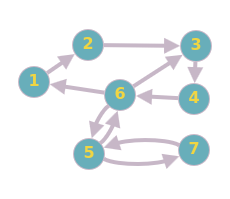
\includegraphics[width=0.7\textwidth]{figures8/digrafo.png}
        \caption{$G$}
    \end{subfigure} 
        \begin{subfigure}[b]{0.45\textwidth}
        \centering
        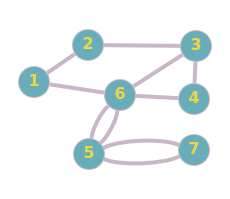
\includegraphics[width=0.7\textwidth]{figures8/Gsubyecente.png}
        \caption{Grafo subyacente de $G$}
         \end{subfigure} 
\end{figure} 
\begin{dfn}
 Un digrafo $D$ es conexo si el multigrafo subyacente de $D$ es conexo
\end{dfn}

\begin{dfn}
 Un digrafo es \textbf{fuertemente conexo} si todo par de nodos del digrafo son mutuamente accesible, o sea si hay camino de uno al otro, y viceversa
\end{dfn}

\begin{figure}[H]
    \centering
    \begin{subfigure}[b]{0.45\textwidth}
        \centering
        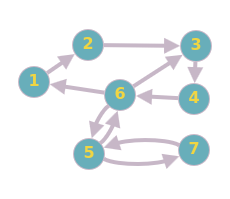
\includegraphics[width=0.7\textwidth]{figures8/digrafo.png}
        \caption{$G$ fuertemente conexo}
    \end{subfigure} 
        \begin{subfigure}[b]{0.45\textwidth}
        \centering
        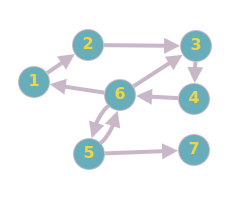
\includegraphics[width=0.7\textwidth]{figures8/NoFConex.png}
        \caption{$G$ no fuertemente conexo}
         \end{subfigure} 

        \caption{En el ejemplo, en a), para todo par de nodos hay un camino por lo que es fuertemente conexo, mientras que en b), desde el nodo $v =7$, no es posible alcanzar ning\'un otro nodo.}
\end{figure} 

\begin{dfn}
 Un grafo es \textbf{orientable} si es posible orientar sus aristas de modo que el digrafo resultante sea fuertemente conexo
\end{dfn}

\begin{teo}
 Sea $G$ un grafo, entonces $G$ es orientable si y solo si $G$ es conexo y no tiene puentes.
\end{teo}

\begin{dem}[$\Rightarrow$]
 
\end{dem}
La demostraci\'on de que $G$ tiene que ser conexo es trival, porque orientar las aristas no va a crear caminos entre las componentes conexas de $G$.

Demostraremos que si $G$ tiene puentes entonces $G$ es no orientable.

Sea $e$ una arista puente tal que $e=\{u,v\}$.

Como $e$ es un puente al removerla $u$ y $v$ quedan en componentes conexas distintas, lo que explica que no exista camino que los conecte. Por lo que si tratamos de orientar 
las aristas de $G-e$ no es posible llegar de $u$ a $v$ (y viceversa). Finalmente la ariasta $\{u,v\}$ se tiene que orientar, si se agrega como $<u,v>$ no habr\'ia camino de $v$ a $u$ en el grafo, an\'alogo para cuando se orienta como $<v,u>$. 
Por tanto  G no es fuertemente conexo luego G no es orientable. \\

\begin{dem}[$\Leftarrow$]
 
\end{dem}

Vamos a utilizar el siguiente lema.

\begin{lem}
 Una arista es puente~(arista de corte) si y solo si no participa en ningún ciclo
\end{lem}

\begin{dem}
Demostración del lema 
\end{dem}


Demostremos que si participa en algún ciclo no es puente.

Sea $e=\{u,v\}\in E(G)$ tal que $e$ participa en el ciclo $c=<u,v,v_1,v_2,\dots,v_k,u>$ entonces $c_1=<v,v_1,v_2,\dots,v_k,u>$ es un camino que contiene a los vértices $u,v$.
Entre todo par de vértices de G, si el camino que los une contiene a la arista $\{u,v\}$, esta puede ser reemplazada por el camino $c_1$, en caso de que no lo contuviera se mantiene igual, por tanto el grafo resultante de eliminar $\{u,v\}$ no varió en la cantidad de componentes conexas, entonces  $e$ no es una arista puente.\\

En el otro sentido, si no es una arista puente entonces participa en algún ciclo.

Sea $e=\{m,v\}\in E(G)$ tal que no es arista puente, en $G-e$ existe un camino que conecta a $m$ con $v$ que no contiene a $e$. 

Sea este $<m,v_1,v_2,\dots,v_k,v>$  luego $c=<m,v_1,v_2,\dots,v_k,v,m>$ es un ciclo al que pertenece $e$.\\

Retornemos a la demostración del teorema.\\

Sea $G'$ el mayor subgrafo orientable de $G$, suponga que hay vértices de $G$ que no pertenecen a $G'$.

Sea entonces $v \in G$ y $v \notin G'$, note que existe $u \in G'$ tal que que $\{u,v\}\in V(G)$ pues $G$ es conexo.

Como $G$ no tiene puentes, por el lema anterior entonces $\{u,v\}$ pertenece a algún ciclo. Sea este $c=<u,v,v_1,v_2,\dots,v_k,u>$, y sea $w$ el primer vértice de $c$ desde $v$ tal que $w \in V(G')$ (Este existe debido a que $u$ pertenece a $G'$ y es el último vértice de $c$).

Entonces se tomará el camino no dirigido de $u$ hacia $w$ y se orientar\'a de la siguiente forma c'$=<u,v,\dots,w>$ tal que los arcos se dirijan en ese sentido.

Note que para todo nodo que pertenece a $G'$ se puede acceder a todo nodo de c'~(puesto que $G'$ es orientable y todo nodo tiene un camino en $G'$ hasta $u$, luego de ahi movi\'endose por $c'$ se alcanzan todos los nodo del camino) y cada nodo de $c'$ puede acceder a $w$, lo que implica que puede acceder a todo nodo de $G'$ y por tanto $G'+c'$ es un subgrafo de $G$ que es orientable y es mayor que $G'$ lo que es una contradicción, luego el mayor subgrafo de $G$ que es orientable es el propio $G$ .

\begin{dfn}
 Un \textbf{torneo} es un digrafo que tiene como grafo subyacente un grafo completo, o sea, un grafo completo orientado
\end{dfn}

\begin{figure}[H]
    \centering
    \begin{subfigure}[b]{0.80\textwidth}
        \centering
        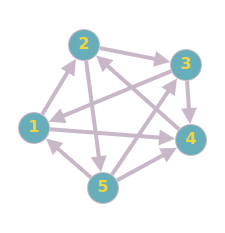
\includegraphics[width=0.4\textwidth]{figures8/torneo.png}
    \end{subfigure} 
    \caption{Ejemplo de Torneo}
\end{figure} 

\begin{teo}
 En todo torneo hay un camino de Hamilton.
\end{teo}

\begin{dem}
 Demostración por inducción el número de nodos
\end{dem}

\textbf{Caso base:} Si $n=1,2$ se cumple.\\

\textbf{Paso inductivo}

Demostremos que si se cumple para $n$ se cumple para $n+1$

Sea $T'=T-{v}$

Note que $T'$ es un torneo, pues tiene $n$ nodos~(hipótesis de inducción), y por tanto existe un camino de Hamilton en $T'$. Sea este $c=<v_1,v_2,\dots,v_n>$.

Ahora:
\begin{itemize}
 \item Si $outdeg(v)=0$ entonces $indeg(v)=n$ luego el camino $<v_1,v_2,\dots,v_n,v>$ es de Hamilton
\end{itemize}

Sea $outdeg(v)=k$ tal que $1 \leq k \leq n$, entonces se pone $v$ delante del primer nodo $v_i$ tal que $<v, v_i> \in T$ (que sabemos existe porque $k > 0$).
Si $v_i = v_1$ entonces se forma el camino de Hamilton $c =<v, v_1,v_2,...,v_n>$, en cualquier otro caso, como $v_i$ es el primero tal que $<v, v_i> \in T$, entonces para $v_{i-1}$ se tiene que $<v_{i-1}, v> \in T$, de donde se forma el camino de Hamilton 
$c = <v_1,...v_{i-1}, v, v_i, ..., v_n>$


\begin{figure}[H]
    \centering
    \begin{subfigure}[b]{0.30\textwidth}
        \centering
        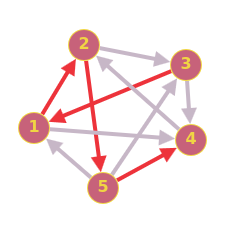
\includegraphics[width=0.7\textwidth]{figures8/Chamilton.png}
    \end{subfigure} 
        \begin{subfigure}[b]{0.55\textwidth}
        \centering
        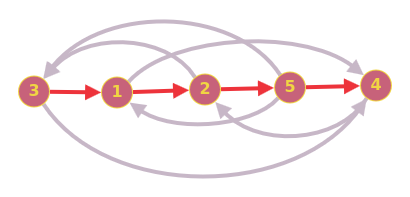
\includegraphics[width=0.7\textwidth]{figures8/HamiltonPath.png}
         \end{subfigure} 

        \caption{Ejemplo de un camino de Hamilton en un Torneo}
\end{figure} 

\begin{teo}
 En un digrafo D se cumple que existe un camino de longitud $\chi(D)-1$
\end{teo}

\begin{dem}
 
\end{dem}


Sea $A$ un conjunto minimal de arcos tal que cuando se elimine el grafo resultante $D-A$ sea acíclico.

Sea $k$ la longitud del camino simple más largo de $D-A$.

Aplíquese la siguiente función de coloración  para los vértices de $D-A$, $f(v)=p$ si $p-1$ es la longitud del camino más largo desde $v$.

Note que para todo vértice $v$ de $D-A$ si $<v,w>\in E(D-A)$ entonces $f(v)\neq f(w)$

Probemos esto, sea $<w,\dots,x>$ de longitud $p-1$, el camino de mayor longitud  desde $w$, n\'otese que ese camino no contiene a $v$ puesto que $D-A$ ac\'iclico.
Luego el camino $<v,w,\dots,x>$ es de longitud $p$, por lo que para $v, \ f(v) \geq p + 1 \neq p = f(w)$ 


Igualmente, se demuestra que para todo nodo $v$ que pertenece a un camino simple se tienen colores distintos.

Como el camino de longitud máxima es de tamaño $k$ entonces para colorear a  $D-A$ bastan $k+1$ colores.

Note que añadir un arco de $A$ necesariamente crea un ciclo, puesto que $A$ era minimal, por tanto si $e=<x,y> \in A$ entonces en $D-A$ existía un camino desde $x$ hasta  $y$, y por tanto sus colores son distintos.

Al añadir todas las aristas de $A$ el grafo continúa pudiendose colorear con $k+1$ colores, entonces $\chi(D)\leq k+1$  luego $k\geq X(D)-1$
  
\end{document} 
